
%% bare_conf.tex
%% V1.4b
%% 2015/08/26
%% by Michael Shell
%% See:
%% http://www.michaelshell.org/
%% for current contact information.
%%
%% This is a skeleton file demonstrating the use of IEEEtran.cls
%% (requires IEEEtran.cls version 1.8b or later) with an IEEE
%% conference paper.
%%
%% Support sites:
%% http://www.michaelshell.org/tex/ieeetran/
%% http://www.ctan.org/pkg/ieeetran
%% and
%% http://www.ieee.org/

%%*************************************************************************
%% Legal Notice:
%% This code is offered as-is without any warranty either expressed or
%% implied; without even the implied warranty of MERCHANTABILITY or
%% FITNESS FOR A PARTICULAR PURPOSE! 
%% User assumes all risk.
%% In no event shall the IEEE or any contributor to this code be liable for
%% any damages or losses, including, but not limited to, incidental,
%% consequential, or any other damages, resulting from the use or misuse
%% of any information contained here.
%%
%% All comments are the opinions of their respective authors and are not
%% necessarily endorsed by the IEEE.
%%
%% This work is distributed under the LaTeX Project Public License (LPPL)
%% ( http://www.latex-project.org/ ) version 1.3, and may be freely used,
%% distributed and modified. A copy of the LPPL, version 1.3, is included
%% in the base LaTeX documentation of all distributions of LaTeX released
%% 2003/12/01 or later.
%% Retain all contribution notices and credits.
%% ** Modified files should be clearly indicated as such, including  **
%% ** renaming them and changing author support contact information. **
%%*************************************************************************


% *** Authors should verify (and, if needed, correct) their LaTeX system  ***
% *** with the testflow diagnostic prior to trusting their LaTeX platform ***
% *** with production work. The IEEE's font choices and paper sizes can   ***
% *** trigger bugs that do not appear when using other class files.       ***                          ***
% The testflow support page is at:
% http://www.michaelshell.org/tex/testflow/



\documentclass[conference]{IEEEtran}
% Some Computer Society conferences also require the compsoc mode option,
% but others use the standard conference format.
%
% If IEEEtran.cls has not been installed into the LaTeX system files,
% manually specify the path to it like:
% \documentclass[conference]{../sty/IEEEtran}





% Some very useful LaTeX packages include:
% (uncomment the ones you want to load)


% *** MISC UTILITY PACKAGES ***
%
%\usepackage{ifpdf}
% Heiko Oberdiek's ifpdf.sty is very useful if you need conditional
% compilation based on whether the output is pdf or dvi.
% usage:
% \ifpdf
%   % pdf code
% \else
%   % dvi code
% \fi
% The latest version of ifpdf.sty can be obtained from:
% http://www.ctan.org/pkg/ifpdf
% Also, note that IEEEtran.cls V1.7 and later provides a builtin
% \ifCLASSINFOpdf conditional that works the same way.
% When switching from latex to pdflatex and vice-versa, the compiler may
% have to be run twice to clear warning/error messages.






% *** CITATION PACKAGES ***
%
%\usepackage{cite}
% cite.sty was written by Donald Arseneau
% V1.6 and later of IEEEtran pre-defines the format of the cite.sty package
% \cite{} output to follow that of the IEEE. Loading the cite package will
% result in citation numbers being automatically sorted and properly
% "compressed/ranged". e.g., [1], [9], [2], [7], [5], [6] without using
% cite.sty will become [1], [2], [5]--[7], [9] using cite.sty. cite.sty's
% \cite will automatically add leading space, if needed. Use cite.sty's
% noadjust option (cite.sty V3.8 and later) if you want to turn this off
% such as if a citation ever needs to be enclosed in parenthesis.
% cite.sty is already installed on most LaTeX systems. Be sure and use
% version 5.0 (2009-03-20) and later if using hyperref.sty.
% The latest version can be obtained at:
% http://www.ctan.org/pkg/cite
% The documentation is contained in the cite.sty file itself.






% *** GRAPHICS RELATED PACKAGES ***
%
\ifCLASSINFOpdf
  % \usepackage[pdftex]{graphicx}
  % declare the path(s) where your graphic files are
  % \graphicspath{{../pdf/}{../jpeg/}}
  % and their extensions so you won't have to specify these with
  % every instance of \includegraphics
  % \DeclareGraphicsExtensions{.pdf,.jpeg,.png}
\else
  % or other class option (dvipsone, dvipdf, if not using dvips). graphicx
  % will default to the driver specified in the system graphics.cfg if no
  % driver is specified.
  % \usepackage[dvips]{graphicx}
  % declare the path(s) where your graphic files are
  % \graphicspath{{../eps/}}
  % and their extensions so you won't have to specify these with
  % every instance of \includegraphics
  % \DeclareGraphicsExtensions{.eps}
\fi
% graphicx was written by David Carlisle and Sebastian Rahtz. It is
% required if you want graphics, photos, etc. graphicx.sty is already
% installed on most LaTeX systems. The latest version and documentation
% can be obtained at: 
% http://www.ctan.org/pkg/graphicx
% Another good source of documentation is "Using Imported Graphics in
% LaTeX2e" by Keith Reckdahl which can be found at:
% http://www.ctan.org/pkg/epslatex
%
% latex, and pdflatex in dvi mode, support graphics in encapsulated
% postscript (.eps) format. pdflatex in pdf mode supports graphics
% in .pdf, .jpeg, .png and .mps (metapost) formats. Users should ensure
% that all non-photo figures use a vector format (.eps, .pdf, .mps) and
% not a bitmapped formats (.jpeg, .png). The IEEE frowns on bitmapped formats
% which can result in "jaggedy"/blurry rendering of lines and letters as
% well as large increases in file sizes.
%
% You can find documentation about the pdfTeX application at:
% http://www.tug.org/applications/pdftex





% *** MATH PACKAGES ***
%
%\usepackage{amsmath}
% A popular package from the American Mathematical Society that provides
% many useful and powerful commands for dealing with mathematics.
%
% Note that the amsmath package sets \interdisplaylinepenalty to 10000
% thus preventing page breaks from occurring within multiline equations. Use:
%\interdisplaylinepenalty=2500
% after loading amsmath to restore such page breaks as IEEEtran.cls normally
% does. amsmath.sty is already installed on most LaTeX systems. The latest
% version and documentation can be obtained at:
% http://www.ctan.org/pkg/amsmath





% *** SPECIALIZED LIST PACKAGES ***
%
%\usepackage{algorithmic}
% algorithmic.sty was written by Peter Williams and Rogerio Brito.
% This package provides an algorithmic environment fo describing algorithms.
% You can use the algorithmic environment in-text or within a figure
% environment to provide for a floating algorithm. Do NOT use the algorithm
% floating environment provided by algorithm.sty (by the same authors) or
% algorithm2e.sty (by Christophe Fiorio) as the IEEE does not use dedicated
% algorithm float types and packages that provide these will not provide
% correct IEEE style captions. The latest version and documentation of
% algorithmic.sty can be obtained at:
% http://www.ctan.org/pkg/algorithms
% Also of interest may be the (relatively newer and more customizable)
% algorithmicx.sty package by Szasz Janos:
% http://www.ctan.org/pkg/algorithmicx




% *** ALIGNMENT PACKAGES ***
%
%\usepackage{array}
% Frank Mittelbach's and David Carlisle's array.sty patches and improves
% the standard LaTeX2e array and tabular environments to provide better
% appearance and additional user controls. As the default LaTeX2e table
% generation code is lacking to the point of almost being broken with
% respect to the quality of the end results, all users are strongly
% advised to use an enhanced (at the very least that provided by array.sty)
% set of table tools. array.sty is already installed on most systems. The
% latest version and documentation can be obtained at:
% http://www.ctan.org/pkg/array


% IEEEtran contains the IEEEeqnarray family of commands that can be used to
% generate multiline equations as well as matrices, tables, etc., of high
% quality.




% *** SUBFIGURE PACKAGES ***
%\ifCLASSOPTIONcompsoc
%  \usepackage[caption=false,font=normalsize,labelfont=sf,textfont=sf]{subfig}
%\else
%  \usepackage[caption=false,font=footnotesize]{subfig}
%\fi
% subfig.sty, written by Steven Douglas Cochran, is the modern replacement
% for subfigure.sty, the latter of which is no longer maintained and is
% incompatible with some LaTeX packages including fixltx2e. However,
% subfig.sty requires and automatically loads Axel Sommerfeldt's caption.sty
% which will override IEEEtran.cls' handling of captions and this will result
% in non-IEEE style figure/table captions. To prevent this problem, be sure
% and invoke subfig.sty's "caption=false" package option (available since
% subfig.sty version 1.3, 2005/06/28) as this is will preserve IEEEtran.cls
% handling of captions.
% Note that the Computer Society format requires a larger sans serif font
% than the serif footnote size font used in traditional IEEE formatting
% and thus the need to invoke different subfig.sty package options depending
% on whether compsoc mode has been enabled.
%
% The latest version and documentation of subfig.sty can be obtained at:
% http://www.ctan.org/pkg/subfig




% *** FLOAT PACKAGES ***
%
%\usepackage{fixltx2e}
% fixltx2e, the successor to the earlier fix2col.sty, was written by
% Frank Mittelbach and David Carlisle. This package corrects a few problems
% in the LaTeX2e kernel, the most notable of which is that in current
% LaTeX2e releases, the ordering of single and double column floats is not
% guaranteed to be preserved. Thus, an unpatched LaTeX2e can allow a
% single column figure to be placed prior to an earlier double column
% figure.
% Be aware that LaTeX2e kernels dated 2015 and later have fixltx2e.sty's
% corrections already built into the system in which case a warning will
% be issued if an attempt is made to load fixltx2e.sty as it is no longer
% needed.
% The latest version and documentation can be found at:
% http://www.ctan.org/pkg/fixltx2e


%\usepackage{stfloats}
% stfloats.sty was written by Sigitas Tolusis. This package gives LaTeX2e
% the ability to do double column floats at the bottom of the page as well
% as the top. (e.g., "\begin{figure*}[!b]" is not normally possible in
% LaTeX2e). It also provides a command:
%\fnbelowfloat
% to enable the placement of footnotes below bottom floats (the standard
% LaTeX2e kernel puts them above bottom floats). This is an invasive package
% which rewrites many portions of the LaTeX2e float routines. It may not work
% with other packages that modify the LaTeX2e float routines. The latest
% version and documentation can be obtained at:
% http://www.ctan.org/pkg/stfloats
% Do not use the stfloats baselinefloat ability as the IEEE does not allow
% \baselineskip to stretch. Authors submitting work to the IEEE should note
% that the IEEE rarely uses double column equations and that authors should try
% to avoid such use. Do not be tempted to use the cuted.sty or midfloat.sty
% packages (also by Sigitas Tolusis) as the IEEE does not format its papers in
% such ways.
% Do not attempt to use stfloats with fixltx2e as they are incompatible.
% Instead, use Morten Hogholm'a dblfloatfix which combines the features
% of both fixltx2e and stfloats:
%
% \usepackage{dblfloatfix}
% The latest version can be found at:
% http://www.ctan.org/pkg/dblfloatfix


\usepackage{natbib}
\usepackage{url}
\usepackage{tikz}
\usetikzlibrary{shapes.geometric, arrows}

\tikzstyle{startstop} = [rectangle, rounded corners, minimum width=3cm, minimum height=1cm,text centered, draw=black, fill=red!30]
\tikzstyle{io} = [trapezium, trapezium left angle=70, trapezium right angle=110, minimum width=3cm, minimum height=1cm, text centered, draw=black, fill=blue!30]
\tikzstyle{process} = [rectangle, minimum width=3cm, minimum height=1cm, text centered, draw=black, fill=orange!30]
\tikzstyle{decision} = [diamond, minimum width=3cm, minimum height=1cm, text centered, draw=black, fill=green!30]
\tikzstyle{arrow} = [thick,->,>=stealth]



% *** PDF, URL AND HYPERLINK PACKAGES ***
%
%\usepackage{url}
% url.sty was written by Donald Arseneau. It provides better support for
% handling and breaking URLs. url.sty is already installed on most LaTeX
% systems. The latest version and documentation can be obtained at:
% http://www.ctan.org/pkg/url
% Basically, \url{my_url_here}.




% *** Do not adjust lengths that control margins, column widths, etc. ***
% *** Do not use packages that alter fonts (such as pslatex).         ***
% There should be no need to do such things with IEEEtran.cls V1.6 and later.
% (Unless specifically asked to do so by the journal or conference you plan
% to submit to, of course. )


% correct bad hyphenation here
\hyphenation{op-tical net-works semi-conduc-tor}


\begin{document}
%
% paper title
% Titles are generally capitalized except for words such as a, an, and, as,
% at, but, by, for, in, nor, of, on, or, the, to and up, which are usually
% not capitalized unless they are the first or last word of the title.
% Linebreaks \\ can be used within to get better formatting as desired.
% Do not put math or special symbols in the title.
\title{Parallel - Face Detection, Recognition and Tracking}


% author names and affiliations
% use a multiple column layout for up to three different
% affiliations
\author{\IEEEauthorblockN{Pawan Singh Negi}
\IEEEauthorblockA{Department of\\Aerospace Engineering\\
Indian Institute of Technology\\
Bombay, Powai 400076\\
Email: pawan2713@gmail.com}
\and
\IEEEauthorblockN{Aarif Shaikh}
\IEEEauthorblockA{Department of\\ CSRE \\
Indian Institute of Technology\\
Bombay, Powai 400076\\
Email: aarifsk1618@gmail.com}
\and
\IEEEauthorblockN{Minnikanti kartheek}
\IEEEauthorblockA{Department of\\ Mechanical Engineering\\
Indian Institute of Technology\\
Bombay, Powai 400076\\
Email: kartheek.minnikanti@iitb.ac.in}}

% conference papers do not typically use \thanks and this command
% is locked out in conference mode. If really needed, such as for
% the acknowledgment of grants, issue a \IEEEoverridecommandlockouts
% after \documentclass

% for over three affiliations, or if they all won't fit within the width
% of the page, use this alternative format:
% 
%\author{\IEEEauthorblockN{Michael Shell\IEEEauthorrefmark{1},
%Homer Simpson\IEEEauthorrefmark{2},
%James Kirk\IEEEauthorrefmark{3}, 
%Montgomery Scott\IEEEauthorrefmark{3} and
%Eldon Tyrell\IEEEauthorrefmark{4}}
%\IEEEauthorblockA{\IEEEauthorrefmark{1}School of Electrical and Computer Engineering\\
%Georgia Institute of Technology,
%Atlanta, Georgia 30332--0250\\ Email: see http://www.michaelshell.org/contact.html}
%\IEEEauthorblockA{\IEEEauthorrefmark{2}Twentieth Century Fox, Springfield, USA\\
%Email: homer@thesimpsons.com}
%\IEEEauthorblockA{\IEEEauthorrefmark{3}Starfleet Academy, San Francisco, California 96678-2391\\
%Telephone: (800) 555--1212, Fax: (888) 555--1212}
%\IEEEauthorblockA{\IEEEauthorrefmark{4}Tyrell Inc., 123 Replicant Street, Los Angeles, California 90210--4321}}




% use for special paper notices
%\IEEEspecialpapernotice{(Invited Paper)}




% make the title area
\maketitle

% As a general rule, do not put math, special symbols or citations
% in the abstract
\begin{abstract}
The goal of this paper is to implement face detection, recognition and tracking in real time using a parallel programming approach. Recently, there has been a lot of interest in this topic due to recent technological advancements which heavily rely on computer vision such as self-driving cars, autonomous quadcopters, and surveillance. However, scaling it to a crowd of faces in real time is challenging due to increased number of faces to be processed. Moreover, algorithms are getting inherently complex, demanding a significant performance overhead. Thus, taking a parallel approach would provide a significant speedup and thus would help improve the performance of inherently complex face detection, recognition and tracking algorithms.
\end{abstract}

% no keywords




% For peer review papers, you can put extra information on the cover
% page as needed:
% \ifCLASSOPTIONpeerreview
% \begin{center} \bfseries EDICS Category: 3-BBND \end{center}
% \fi
%
% For peerreview papers, this IEEEtran command inserts a page break and
% creates the second title. It will be ignored for other modes.
\IEEEpeerreviewmaketitle



\section{Introduction}
Face detection, recognition and tracking are one of the most researched topic in computer vision. In this report we have used openCV, an open-source library for computer vision to perform detection, recognition and tracking. OpenCV provides various different algorithms for detection, recognition and tracking. Instead of having all the algorithms in one library one have to work to connect detection to recognition and  recognition to tracking of an object. In this program, we started by writing a serial code which includes making database to recognize all the team members. In the second phase we parallelized the program using the inbuilt functions enabling it to use the GPU in the machine. The report consists of the overall flow of the program, detection algorithms, recognition algorithms, object tracking, parallel implementation and results.

\section{Overall flow}
\begin{figure}[h!]
	\centering
	\resizebox{9cm}{4cm}{
	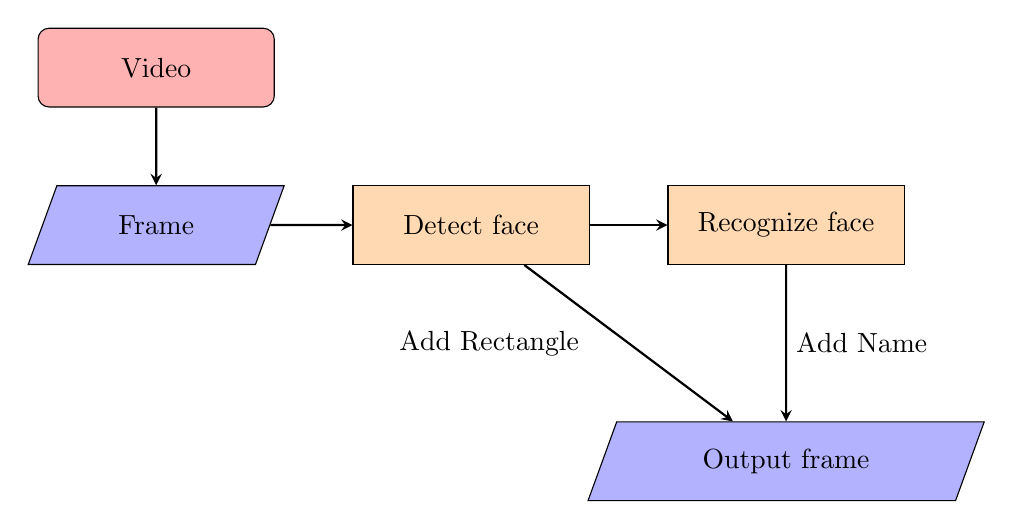
\begin{tikzpicture}[node distance=2cm]
	
	\node (start) [startstop] {Video};
	\node (frame) [io, below of=start] {Frame};
	\node (detect) [process, right of=frame, xshift=2cm] {Detect face};
	\node (recognize) [process, right of=detect, xshift=2cm] {Recognize face};
	\node (outframe) [io, below of=recognize , yshift=-1cm] {Output frame};
	
	\draw [arrow] (start) -- (frame);
	\draw [arrow] (frame) -- (detect);
	\draw [arrow] (detect) -- (recognize);
	\draw [arrow] (detect) -- node[anchor=east , xshift=-0.5cm] {Add Rectangle} (outframe);
	\draw [arrow] (recognize) -- node[anchor=west] {Add Name} (outframe);
	
	\end{tikzpicture}
}
	\caption{Flowchart}
	\label{flow}
\end{figure}
In the Figure \ref{flow}, the video is the starting point. One frame is taken at a time which goes to the Detect face block. Detection of face is performed. Here it is possible to detect multiple faces, if present. It gives cropped faces to the recognize block. In the recognize block, using the training faces it tries to recognize the face. If a match is found, it returns a label which in turn give a name to the face. Detect face provides a frame to the output frame. Thus the output frame contains the face name and a box around it.

\section{Algorithms in OpenCV}
OpenCV provides various algorithms for detection, recognition and tracking. We studied and compared all of them. Depending upon the speed and accuracy we chose one of them.

\subsection{Detection Algorithms}

\subsubsection{Viola Jones Face detection algorithm}
\begin{itemize}
	\item It was the first framework to provide competitive object detection rates in real time \cite{facedet}. 
	\item It was proposed by Viola and Jones (2001) \cite{990517} and was found to present high accuracy compared to existing algorithms.
	\item It was found to be suitable for real time detection as it had low latency.
	\item A cascade of classifiers can be built upon it which would minimize computation time and improve face detection accuracy.
	\item It takes a long time to train the model.
	\item It can detect a limited number of head poses/orientations.
	\item It does not detect dark faces.
\end{itemize}

\subsubsection{Local Binary Pattern}
\begin{itemize}
	\item Local Binary Pattern was found to be Extremely effective in describing image texture features \cite{10.1007/978-981-10-5272-9_20}.
	\item It has use in texture analysis, image retrievals, face recognition and image segmentation. 
	\item It tracks the movement of an object by using background subtraction. 
	\item It is computationally simple and easy to implement. 
	\item It is tolerant to illumination changes.
	\item Using large local regions increases errors.
	\item It is robust but not accurate.
	\item It is suitable only for binary and grayscale images.	
\end{itemize}

\subsubsection{AdaBoost Algorithm}
\begin{itemize}
	\item it is sensitive to noisy data, hence returns a suboptimal solution \cite{10.1007/978-981-10-5272-9_20}.
	\item It is adaptive, one weak classifier added in each iteration.
	\item It does not over-fit to the object in training data set. 
	\item It has a simple implementation.
	\item The results are heavily dependent on the quality of the training data in terms of interclass variability and size of the datasets.
	\item It is very slow to train.
	
\end{itemize}
Haar cacade classifiers are implemented upon the Viola-Jones algorithm. A trained model of it is present in OpenCV library. The good performance achieved compared to other techniques makes it appropriate for solving the current problem, and the same is used in this program.
\subsection{Recognition Algorithms}

\subsubsection{Eigenface Method}
\begin{itemize}
	\item This method uses principal component analysis (PCA) which returns a linear combination of data while maximizing the total variance among all the training sets \cite{facerec}. 
	\item From the image database a covariance matrix is calculated, for which eigenvalues and eigenvectors are calculated. 
	\item Through PCA, any face can be represented as linear combination of derived models.
	\item Any face is represented as
	\begin{equation}
		face = \mu + \sum_{i=1}^{N} x_i \nu_{i}
	\end{equation}
	where $\mu$ is meanface, $x_i$ is the weight and $\nu_{i}$ is the eigenface.                                          
	\item Once eigenfaces of trained data set is formed, it can be used to recognize new image of any face in the database in real time.
\end{itemize}

\subsubsection{Fisherface Method}
\begin{itemize}
	\item This method uses Linear Discriminant Analysis \cite{facerec}. 
	\item It tries to develop a model which maximizes the ratio of between-classes to within-classes variance.
	\item It is more class specific approach.
\end{itemize}

\subsubsection{Local Binary Pattern Histogram Method (LBPH)}
\begin{itemize}
	\item It uses local binary patterns to recognize face features \cite{facerec}.
	\item This method can differentiate features locally in an image based on pixels relative to neighbours. 
	\item This information is used to plot histograms based on frequency of the binary number which gives a model from trained dataset. 
	\item The advantage of this method to above mentioned method is that the variation in illumination effects can be managed as it is taking data relative to each other. 
	\item It is more robust compared to other methods. 
	\item The histograms that we got from training dataset is used to identify new image of any face in the database.
\end{itemize}
On looking at the advantages of LBPH method to recognize face at all illumination conditions and robustness, we have chosen LBPH method for face recognition.

\subsection{Tracking Algorithms}

We found that tracking in openCV is a loose end. It relies on detection \cite{facetrack}. The following are the steps involved in tracking:
\begin{enumerate}
	\item Detect eyes in the frame.
	\item Calculate angle made with the horizontal.
	\item Rotate the frame with the calculated angle.
	\item Detect face.
	\item Track face.
	\item If track failed go to 1.
\end{enumerate}

\section{Results}
We successfully implemented the serial code for detection and recognition. Recognition also includes making the database of faces. We made database of all the team members and tried to recognize ourselves using the webcam feed. The result is given in the Figure \ref{res}.
\begin{figure}[h!]
	\centering
	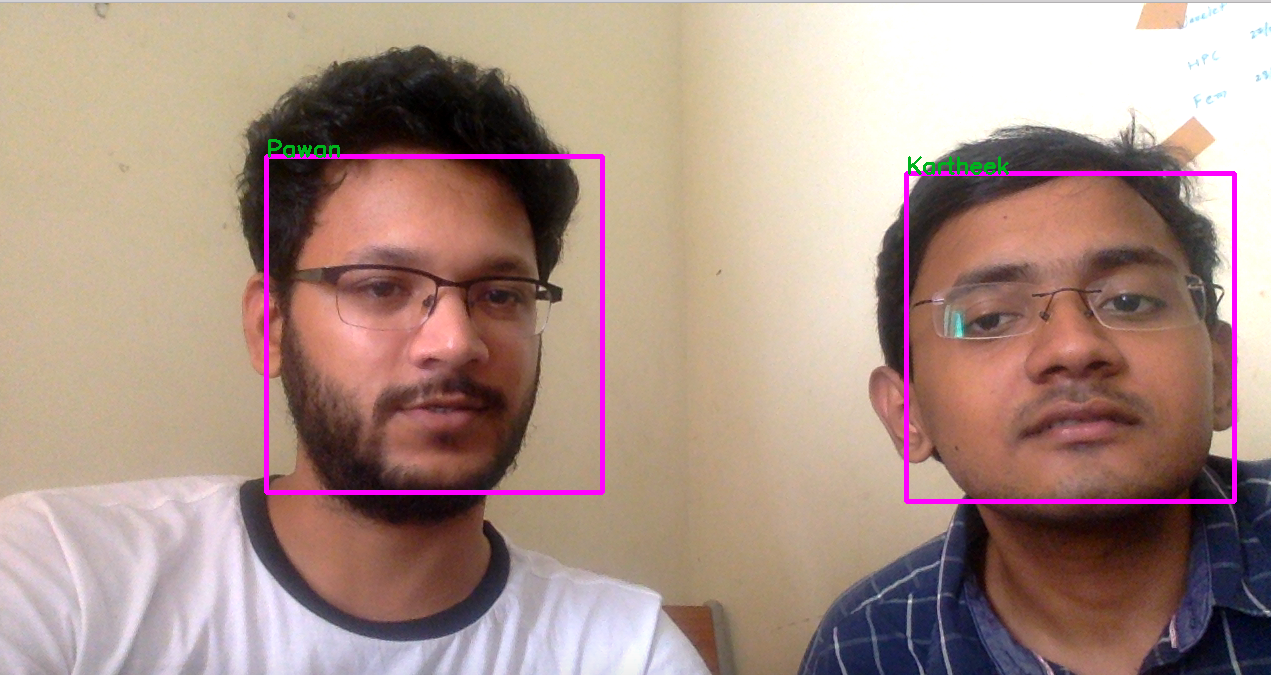
\includegraphics[scale=0.2]{./images/res.png}
	\caption{Recognized faces with label}
	\label{res}
\end{figure}

\section{Parallel Implementation}
The video input is 14.5 fps thus we need to have a speed of detection and recognition to be 0.07 seconds. For serial code we were getting 0.41 seconds, which results in lag between video feed and recognition output frame. We needed to speed up the process, thus we used the inbuilt functionality of openCV for parallelization. OpenCV provides two classes to store frames namely Mat and UMat \cite{opencl}. 
\begin{figure}[h!]
	\centering
	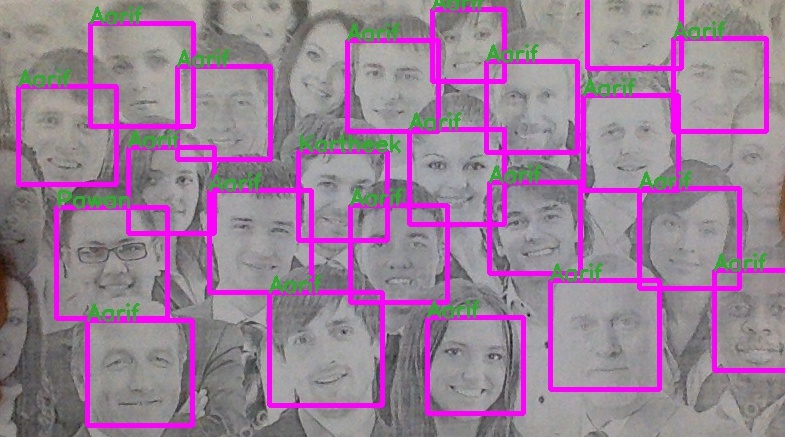
\includegraphics[scale=0.3]{./images/mul.jpg}
	\caption{Multiples faces detected}
	\label{mul}
\end{figure}
If a frame is declared as UMat OpenCV automatically do all the operations in the available GPU. There are some exceptions like imread and imshow function which do not recognize UMat, there we have made necessary conversion from UMat to Mat. The parallel implementation helps us to detect and recognize multiple faces with some speedup. The multiple face output is shown in the Figure \ref{mul}. We compared the results of the serial code with the parallel code as shown in the Figure \ref{plot}
\begin{figure}[h!]
	\centering
	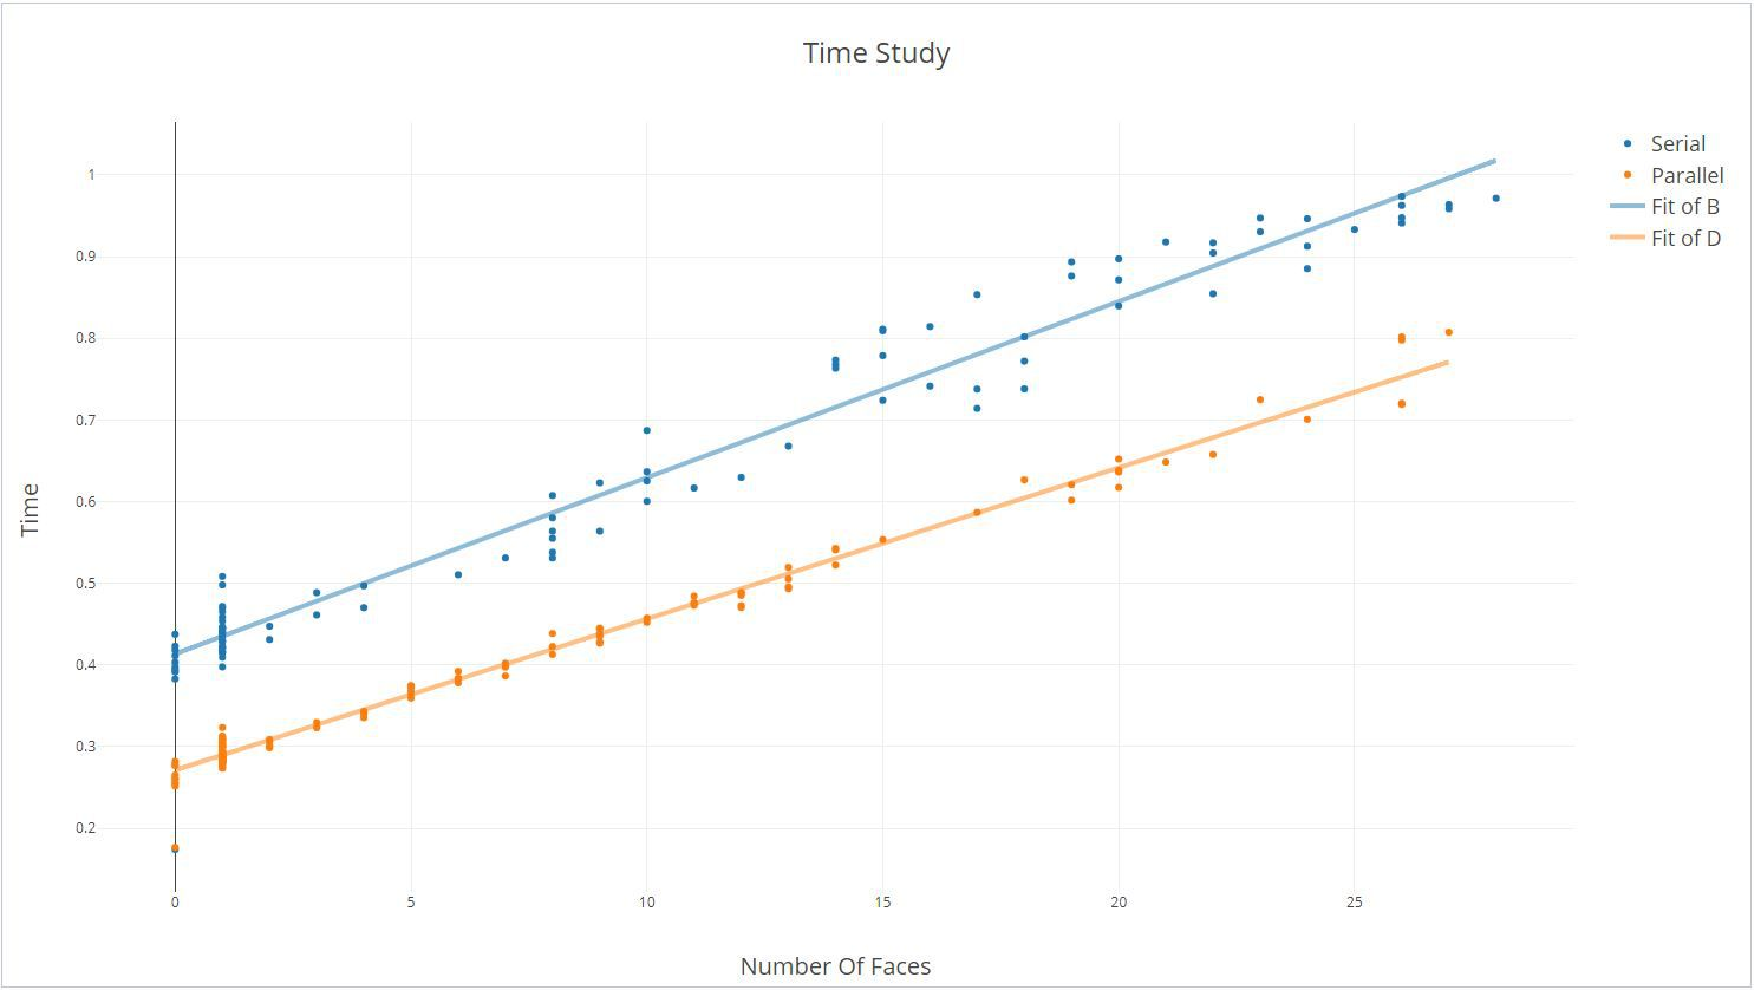
\includegraphics[scale=0.6]{./images/plot.pdf}
	\caption{Detected face vs time}
	\label{plot}
\end{figure}


% An example of a floating figure using the graphicx package.
% Note that \label must occur AFTER (or within) \caption.
% For figures, \caption should occur after the \includegraphics.
% Note that IEEEtran v1.7 and later has special internal code that
% is designed to preserve the operation of \label within \caption
% even when the captionsoff option is in effect. However, because
% of issues like this, it may be the safest practice to put all your
% \label just after \caption rather than within \caption{}.
%
% Reminder: the "draftcls" or "draftclsnofoot", not "draft", class
% option should be used if it is desired that the figures are to be
% displayed while in draft mode.
%
%\begin{figure}[!t]
%\centering
%\includegraphics[width=2.5in]{myfigure}
% where an .eps filename suffix will be assumed under latex, 
% and a .pdf suffix will be assumed for pdflatex; or what has been declared
% via \DeclareGraphicsExtensions.
%\caption{Simulation results for the network.}
%\label{fig_sim}
%\end{figure}

% Note that the IEEE typically puts floats only at the top, even when this
% results in a large percentage of a column being occupied by floats.


% An example of a double column floating figure using two subfigures.
% (The subfig.sty package must be loaded for this to work.)
% The subfigure \label commands are set within each subfloat command,
% and the \label for the overall figure must come after \caption.
% \hfil is used as a separator to get equal spacing.
% Watch out that the combined width of all the subfigures on a 
% line do not exceed the text width or a line break will occur.
%
%\begin{figure*}[!t]
%\centering
%\subfloat[Case I]{\includegraphics[width=2.5in]{box}%
%\label{fig_first_case}}
%\hfil
%\subfloat[Case II]{\includegraphics[width=2.5in]{box}%
%\label{fig_second_case}}
%\caption{Simulation results for the network.}
%\label{fig_sim}
%\end{figure*}
%
% Note that often IEEE papers with subfigures do not employ subfigure
% captions (using the optional argument to \subfloat[]), but instead will
% reference/describe all of them (a), (b), etc., within the main caption.
% Be aware that for subfig.sty to generate the (a), (b), etc., subfigure
% labels, the optional argument to \subfloat must be present. If a
% subcaption is not desired, just leave its contents blank,
% e.g., \subfloat[].


% An example of a floating table. Note that, for IEEE style tables, the
% \caption command should come BEFORE the table and, given that table
% captions serve much like titles, are usually capitalized except for words
% such as a, an, and, as, at, but, by, for, in, nor, of, on, or, the, to
% and up, which are usually not capitalized unless they are the first or
% last word of the caption. Table text will default to \footnotesize as
% the IEEE normally uses this smaller font for tables.
% The \label must come after \caption as always.
%
%\begin{table}[!t]
%% increase table row spacing, adjust to taste
%\renewcommand{\arraystretch}{1.3}
% if using array.sty, it might be a good idea to tweak the value of
% \extrarowheight as needed to properly center the text within the cells
%\caption{An Example of a Table}
%\label{table_example}
%\centering
%% Some packages, such as MDW tools, offer better commands for making tables
%% than the plain LaTeX2e tabular which is used here.
%\begin{tabular}{|c||c|}
%\hline
%One & Two\\
%\hline
%Three & Four\\
%\hline
%\end{tabular}
%\end{table}


% Note that the IEEE does not put floats in the very first column
% - or typically anywhere on the first page for that matter. Also,
% in-text middle ("here") positioning is typically not used, but it
% is allowed and encouraged for Computer Society conferences (but
% not Computer Society journals). Most IEEE journals/conferences use
% top floats exclusively. 
% Note that, LaTeX2e, unlike IEEE journals/conferences, places
% footnotes above bottom floats. This can be corrected via the
% \fnbelowfloat command of the stfloats package.




\section{Conclusion}
We used openCV library to detect and recognize faces in the video feed from the webcam. We also attempted to track the face in the frame which would have resulted in a significant speedup as it decreases the computational load. We used Github for the version control of the project. The link for the project is \url{https://github.com/psnbaba/HPC_project}. We used Doxygen type commenting style to enable document generation for the code base which will in turn help others to develop over the existing code base.




% conference papers do not normally have an appendix


% use section* for acknowledgment





% trigger a \newpage just before the given reference
% number - used to balance the columns on the last page
% adjust value as needed - may need to be readjusted if
% the document is modified later
%\IEEEtriggeratref{8}
% The "triggered" command can be changed if desired:
%\IEEEtriggercmd{\enlargethispage{-5in}}

% references section

% can use a bibliography generated by BibTeX as a .bbl file
% BibTeX documentation can be easily obtained at:
% http://mirror.ctan.org/biblio/bibtex/contrib/doc/
% The IEEEtran BibTeX style support page is at:
% http://www.michaelshell.org/tex/ieeetran/bibtex/
%\bibliographystyle{IEEEtran}
% argument is your BibTeX string definitions and bibliography database(s)
%\bibliography{IEEEabrv,../bib/paper}
%
% <OR> manually copy in the resultant .bbl file
% set second argument of \begin to the number of references
% (used to reserve space for the reference number labels box)

\bibliographystyle{plain}
\bibliography{./ref}







% that's all folks
\end{document}


